% Created by tikzDevice version 0.8.1 on 2015-11-17 12:15:23
% !TEX encoding = UTF-8 Unicode
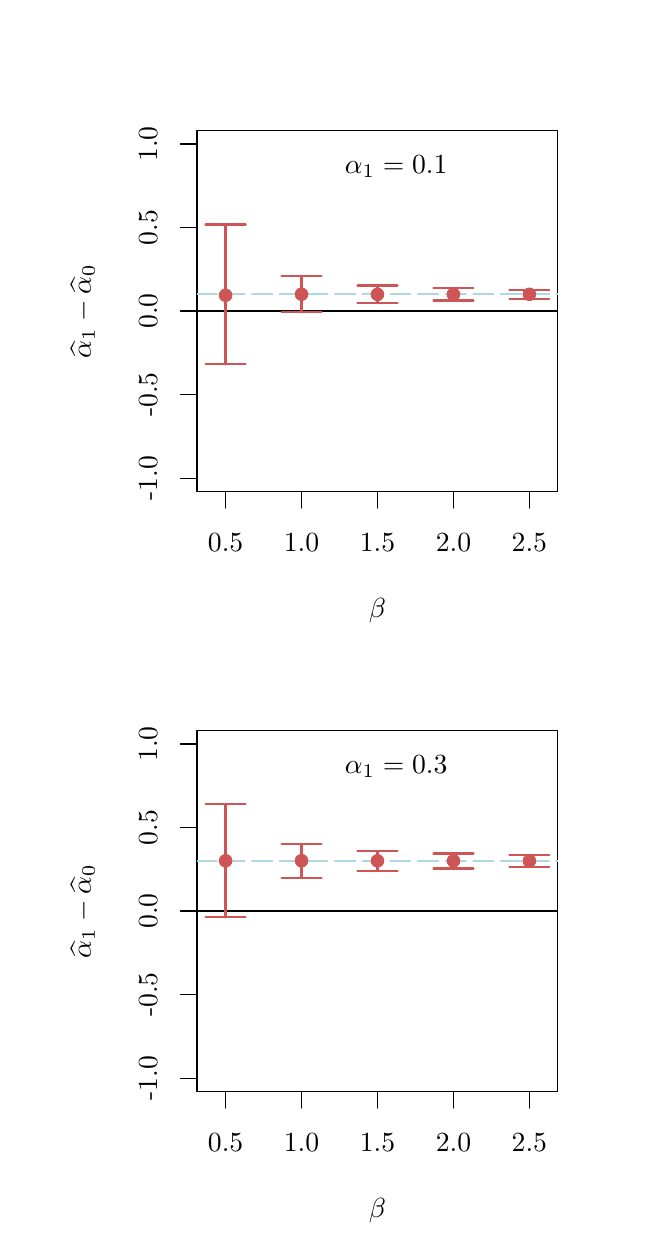
\begin{tikzpicture}[x=1pt,y=1pt]
\definecolor{fillColor}{RGB}{255,255,255}
\path[use as bounding box,fill=fillColor,fill opacity=0.00] (0,0) rectangle (216.81,433.62);
\begin{scope}
\path[clip] ( 61.20,266.01) rectangle (191.61,396.42);
\definecolor{drawColor}{RGB}{255,255,255}
\definecolor{fillColor}{RGB}{255,255,255}

\path[draw=drawColor,line width= 0.4pt,line join=round,line cap=round,fill=fillColor] ( 71.52,336.92) circle (  2.25);

\path[draw=drawColor,line width= 0.4pt,line join=round,line cap=round,fill=fillColor] ( 98.96,337.30) circle (  2.25);

\path[draw=drawColor,line width= 0.4pt,line join=round,line cap=round,fill=fillColor] (126.40,337.24) circle (  2.25);

\path[draw=drawColor,line width= 0.4pt,line join=round,line cap=round,fill=fillColor] (153.85,337.26) circle (  2.25);

\path[draw=drawColor,line width= 0.4pt,line join=round,line cap=round,fill=fillColor] (181.29,337.28) circle (  2.25);
\end{scope}
\begin{scope}
\path[clip] (  0.00,  0.00) rectangle (216.81,433.62);
\definecolor{drawColor}{RGB}{0,0,0}

\path[draw=drawColor,line width= 0.4pt,line join=round,line cap=round] ( 71.52,266.01) -- (181.29,266.01);

\path[draw=drawColor,line width= 0.4pt,line join=round,line cap=round] ( 71.52,266.01) -- ( 71.52,260.01);

\path[draw=drawColor,line width= 0.4pt,line join=round,line cap=round] ( 98.96,266.01) -- ( 98.96,260.01);

\path[draw=drawColor,line width= 0.4pt,line join=round,line cap=round] (126.40,266.01) -- (126.40,260.01);

\path[draw=drawColor,line width= 0.4pt,line join=round,line cap=round] (153.85,266.01) -- (153.85,260.01);

\path[draw=drawColor,line width= 0.4pt,line join=round,line cap=round] (181.29,266.01) -- (181.29,260.01);

\node[text=drawColor,anchor=base,inner sep=0pt, outer sep=0pt, scale=  1.00] at ( 71.52,244.41) {0.5};

\node[text=drawColor,anchor=base,inner sep=0pt, outer sep=0pt, scale=  1.00] at ( 98.96,244.41) {1.0};

\node[text=drawColor,anchor=base,inner sep=0pt, outer sep=0pt, scale=  1.00] at (126.40,244.41) {1.5};

\node[text=drawColor,anchor=base,inner sep=0pt, outer sep=0pt, scale=  1.00] at (153.85,244.41) {2.0};

\node[text=drawColor,anchor=base,inner sep=0pt, outer sep=0pt, scale=  1.00] at (181.29,244.41) {2.5};

\path[draw=drawColor,line width= 0.4pt,line join=round,line cap=round] ( 61.20,270.84) -- ( 61.20,391.59);

\path[draw=drawColor,line width= 0.4pt,line join=round,line cap=round] ( 61.20,270.84) -- ( 55.20,270.84);

\path[draw=drawColor,line width= 0.4pt,line join=round,line cap=round] ( 61.20,301.03) -- ( 55.20,301.03);

\path[draw=drawColor,line width= 0.4pt,line join=round,line cap=round] ( 61.20,331.22) -- ( 55.20,331.22);

\path[draw=drawColor,line width= 0.4pt,line join=round,line cap=round] ( 61.20,361.40) -- ( 55.20,361.40);

\path[draw=drawColor,line width= 0.4pt,line join=round,line cap=round] ( 61.20,391.59) -- ( 55.20,391.59);

\node[text=drawColor,rotate= 90.00,anchor=base,inner sep=0pt, outer sep=0pt, scale=  1.00] at ( 46.80,270.84) {-1.0};

\node[text=drawColor,rotate= 90.00,anchor=base,inner sep=0pt, outer sep=0pt, scale=  1.00] at ( 46.80,301.03) {-0.5};

\node[text=drawColor,rotate= 90.00,anchor=base,inner sep=0pt, outer sep=0pt, scale=  1.00] at ( 46.80,331.22) {0.0};

\node[text=drawColor,rotate= 90.00,anchor=base,inner sep=0pt, outer sep=0pt, scale=  1.00] at ( 46.80,361.40) {0.5};

\node[text=drawColor,rotate= 90.00,anchor=base,inner sep=0pt, outer sep=0pt, scale=  1.00] at ( 46.80,391.59) {1.0};

\path[draw=drawColor,line width= 0.4pt,line join=round,line cap=round] ( 61.20,266.01) --
	(191.61,266.01) --
	(191.61,396.42) --
	( 61.20,396.42) --
	( 61.20,266.01);
\end{scope}
\begin{scope}
\path[clip] (  0.00,216.81) rectangle (216.81,433.62);
\definecolor{drawColor}{RGB}{0,0,0}

\node[text=drawColor,anchor=base,inner sep=0pt, outer sep=0pt, scale=  1.00] at (126.41,220.41) {$\beta$};

\node[text=drawColor,rotate= 90.00,anchor=base,inner sep=0pt, outer sep=0pt, scale=  1.00] at ( 22.80,331.22) {$\widehat{\alpha}_1 - \widehat{\alpha}_0$};
\end{scope}
\begin{scope}
\path[clip] ( 61.20,266.01) rectangle (191.61,396.42);
\definecolor{drawColor}{RGB}{0,0,0}

\node[text=drawColor,anchor=base west,inner sep=0pt, outer sep=0pt, scale=  1.00] at (114.66,380.98) {$\alpha_1=0.1$};
\definecolor{drawColor}{RGB}{173,216,230}

\path[draw=drawColor,line width= 0.8pt,dash pattern=on 7pt off 3pt ,line join=round,line cap=round] ( 61.20,337.25) -- (191.61,337.25);

\path[draw=drawColor,line width= 0.8pt,dash pattern=on 7pt off 3pt ,line join=round,line cap=round] ( 61.20,337.25) -- (191.61,337.25);

\path[draw=drawColor,line width= 0.8pt,dash pattern=on 7pt off 3pt ,line join=round,line cap=round] ( 61.20,337.25) -- (191.61,337.25);

\path[draw=drawColor,line width= 0.8pt,dash pattern=on 7pt off 3pt ,line join=round,line cap=round] ( 61.20,337.25) -- (191.61,337.25);

\path[draw=drawColor,line width= 0.8pt,dash pattern=on 7pt off 3pt ,line join=round,line cap=round] ( 61.20,337.25) -- (191.61,337.25);
\definecolor{drawColor}{RGB}{0,0,0}

\path[draw=drawColor,line width= 0.4pt,line join=round,line cap=round] ( 61.20,331.22) -- (191.61,331.22);
\definecolor{drawColor}{RGB}{205,85,85}

\path[draw=drawColor,line width= 0.8pt,line join=round,line cap=round] ( 71.52,311.95) -- ( 71.52,362.46);

\path[draw=drawColor,line width= 0.8pt,line join=round,line cap=round] ( 64.29,311.95) --
	( 71.52,311.95) --
	( 78.75,311.95);

\path[draw=drawColor,line width= 0.8pt,line join=round,line cap=round] ( 78.75,362.46) --
	( 71.52,362.46) --
	( 64.29,362.46);

\path[draw=drawColor,line width= 0.8pt,line join=round,line cap=round] ( 98.96,330.75) -- ( 98.96,343.92);

\path[draw=drawColor,line width= 0.8pt,line join=round,line cap=round] ( 91.73,330.75) --
	( 98.96,330.75) --
	(106.19,330.75);

\path[draw=drawColor,line width= 0.8pt,line join=round,line cap=round] (106.19,343.92) --
	( 98.96,343.92) --
	( 91.73,343.92);

\path[draw=drawColor,line width= 0.8pt,line join=round,line cap=round] (126.40,334.02) -- (126.40,340.48);

\path[draw=drawColor,line width= 0.8pt,line join=round,line cap=round] (119.18,334.02) --
	(126.40,334.02) --
	(133.63,334.02);

\path[draw=drawColor,line width= 0.8pt,line join=round,line cap=round] (133.63,340.48) --
	(126.40,340.48) --
	(119.18,340.48);

\path[draw=drawColor,line width= 0.8pt,line join=round,line cap=round] (153.85,335.05) -- (153.85,339.44);

\path[draw=drawColor,line width= 0.8pt,line join=round,line cap=round] (146.62,335.05) --
	(153.85,335.05) --
	(161.08,335.05);

\path[draw=drawColor,line width= 0.8pt,line join=round,line cap=round] (161.08,339.44) --
	(153.85,339.44) --
	(146.62,339.44);

\path[draw=drawColor,line width= 0.8pt,line join=round,line cap=round] (181.29,335.58) -- (181.29,338.95);

\path[draw=drawColor,line width= 0.8pt,line join=round,line cap=round] (174.06,335.58) --
	(181.29,335.58) --
	(188.52,335.58);

\path[draw=drawColor,line width= 0.8pt,line join=round,line cap=round] (188.52,338.95) --
	(181.29,338.95) --
	(174.06,338.95);
\definecolor{fillColor}{RGB}{205,85,85}

\path[draw=drawColor,line width= 0.4pt,line join=round,line cap=round,fill=fillColor] ( 71.52,336.92) circle (  2.25);

\path[draw=drawColor,line width= 0.4pt,line join=round,line cap=round,fill=fillColor] ( 98.96,337.30) circle (  2.25);

\path[draw=drawColor,line width= 0.4pt,line join=round,line cap=round,fill=fillColor] (126.40,337.24) circle (  2.25);

\path[draw=drawColor,line width= 0.4pt,line join=round,line cap=round,fill=fillColor] (153.85,337.26) circle (  2.25);

\path[draw=drawColor,line width= 0.4pt,line join=round,line cap=round,fill=fillColor] (181.29,337.28) circle (  2.25);
\end{scope}
\begin{scope}
\path[clip] ( 61.20, 49.20) rectangle (191.61,179.61);
\definecolor{drawColor}{RGB}{255,255,255}
\definecolor{fillColor}{RGB}{255,255,255}

\path[draw=drawColor,line width= 0.4pt,line join=round,line cap=round,fill=fillColor] ( 71.52,132.57) circle (  2.25);

\path[draw=drawColor,line width= 0.4pt,line join=round,line cap=round,fill=fillColor] ( 98.96,132.60) circle (  2.25);

\path[draw=drawColor,line width= 0.4pt,line join=round,line cap=round,fill=fillColor] (126.40,132.56) circle (  2.25);

\path[draw=drawColor,line width= 0.4pt,line join=round,line cap=round,fill=fillColor] (153.85,132.54) circle (  2.25);

\path[draw=drawColor,line width= 0.4pt,line join=round,line cap=round,fill=fillColor] (181.29,132.52) circle (  2.25);
\end{scope}
\begin{scope}
\path[clip] (  0.00,  0.00) rectangle (216.81,433.62);
\definecolor{drawColor}{RGB}{0,0,0}

\path[draw=drawColor,line width= 0.4pt,line join=round,line cap=round] ( 71.52, 49.20) -- (181.29, 49.20);

\path[draw=drawColor,line width= 0.4pt,line join=round,line cap=round] ( 71.52, 49.20) -- ( 71.52, 43.20);

\path[draw=drawColor,line width= 0.4pt,line join=round,line cap=round] ( 98.96, 49.20) -- ( 98.96, 43.20);

\path[draw=drawColor,line width= 0.4pt,line join=round,line cap=round] (126.40, 49.20) -- (126.40, 43.20);

\path[draw=drawColor,line width= 0.4pt,line join=round,line cap=round] (153.85, 49.20) -- (153.85, 43.20);

\path[draw=drawColor,line width= 0.4pt,line join=round,line cap=round] (181.29, 49.20) -- (181.29, 43.20);

\node[text=drawColor,anchor=base,inner sep=0pt, outer sep=0pt, scale=  1.00] at ( 71.52, 27.60) {0.5};

\node[text=drawColor,anchor=base,inner sep=0pt, outer sep=0pt, scale=  1.00] at ( 98.96, 27.60) {1.0};

\node[text=drawColor,anchor=base,inner sep=0pt, outer sep=0pt, scale=  1.00] at (126.40, 27.60) {1.5};

\node[text=drawColor,anchor=base,inner sep=0pt, outer sep=0pt, scale=  1.00] at (153.85, 27.60) {2.0};

\node[text=drawColor,anchor=base,inner sep=0pt, outer sep=0pt, scale=  1.00] at (181.29, 27.60) {2.5};

\path[draw=drawColor,line width= 0.4pt,line join=round,line cap=round] ( 61.20, 54.03) -- ( 61.20,174.78);

\path[draw=drawColor,line width= 0.4pt,line join=round,line cap=round] ( 61.20, 54.03) -- ( 55.20, 54.03);

\path[draw=drawColor,line width= 0.4pt,line join=round,line cap=round] ( 61.20, 84.22) -- ( 55.20, 84.22);

\path[draw=drawColor,line width= 0.4pt,line join=round,line cap=round] ( 61.20,114.41) -- ( 55.20,114.41);

\path[draw=drawColor,line width= 0.4pt,line join=round,line cap=round] ( 61.20,144.59) -- ( 55.20,144.59);

\path[draw=drawColor,line width= 0.4pt,line join=round,line cap=round] ( 61.20,174.78) -- ( 55.20,174.78);

\node[text=drawColor,rotate= 90.00,anchor=base,inner sep=0pt, outer sep=0pt, scale=  1.00] at ( 46.80, 54.03) {-1.0};

\node[text=drawColor,rotate= 90.00,anchor=base,inner sep=0pt, outer sep=0pt, scale=  1.00] at ( 46.80, 84.22) {-0.5};

\node[text=drawColor,rotate= 90.00,anchor=base,inner sep=0pt, outer sep=0pt, scale=  1.00] at ( 46.80,114.41) {0.0};

\node[text=drawColor,rotate= 90.00,anchor=base,inner sep=0pt, outer sep=0pt, scale=  1.00] at ( 46.80,144.59) {0.5};

\node[text=drawColor,rotate= 90.00,anchor=base,inner sep=0pt, outer sep=0pt, scale=  1.00] at ( 46.80,174.78) {1.0};

\path[draw=drawColor,line width= 0.4pt,line join=round,line cap=round] ( 61.20, 49.20) --
	(191.61, 49.20) --
	(191.61,179.61) --
	( 61.20,179.61) --
	( 61.20, 49.20);
\end{scope}
\begin{scope}
\path[clip] (  0.00,  0.00) rectangle (216.81,216.81);
\definecolor{drawColor}{RGB}{0,0,0}

\node[text=drawColor,anchor=base,inner sep=0pt, outer sep=0pt, scale=  1.00] at (126.41,  3.60) {$\beta$};

\node[text=drawColor,rotate= 90.00,anchor=base,inner sep=0pt, outer sep=0pt, scale=  1.00] at ( 22.80,114.41) {$\widehat{\alpha}_1 - \widehat{\alpha}_0$};
\end{scope}
\begin{scope}
\path[clip] ( 61.20, 49.20) rectangle (191.61,179.61);
\definecolor{drawColor}{RGB}{0,0,0}

\node[text=drawColor,anchor=base west,inner sep=0pt, outer sep=0pt, scale=  1.00] at (114.66,164.17) {$\alpha_1=0.3$};
\definecolor{drawColor}{RGB}{173,216,230}

\path[draw=drawColor,line width= 0.8pt,dash pattern=on 7pt off 3pt ,line join=round,line cap=round] ( 61.20,132.52) -- (191.61,132.52);

\path[draw=drawColor,line width= 0.8pt,dash pattern=on 7pt off 3pt ,line join=round,line cap=round] ( 61.20,132.52) -- (191.61,132.52);

\path[draw=drawColor,line width= 0.8pt,dash pattern=on 7pt off 3pt ,line join=round,line cap=round] ( 61.20,132.52) -- (191.61,132.52);

\path[draw=drawColor,line width= 0.8pt,dash pattern=on 7pt off 3pt ,line join=round,line cap=round] ( 61.20,132.52) -- (191.61,132.52);

\path[draw=drawColor,line width= 0.8pt,dash pattern=on 7pt off 3pt ,line join=round,line cap=round] ( 61.20,132.52) -- (191.61,132.52);
\definecolor{drawColor}{RGB}{0,0,0}

\path[draw=drawColor,line width= 0.4pt,line join=round,line cap=round] ( 61.20,114.41) -- (191.61,114.41);
\definecolor{drawColor}{RGB}{205,85,85}

\path[draw=drawColor,line width= 0.8pt,line join=round,line cap=round] ( 71.52,112.14) -- ( 71.52,152.95);

\path[draw=drawColor,line width= 0.8pt,line join=round,line cap=round] ( 64.29,112.14) --
	( 71.52,112.14) --
	( 78.75,112.14);

\path[draw=drawColor,line width= 0.8pt,line join=round,line cap=round] ( 78.75,152.95) --
	( 71.52,152.95) --
	( 64.29,152.95);

\path[draw=drawColor,line width= 0.8pt,line join=round,line cap=round] ( 98.96,126.34) -- ( 98.96,138.53);

\path[draw=drawColor,line width= 0.8pt,line join=round,line cap=round] ( 91.73,126.34) --
	( 98.96,126.34) --
	(106.19,126.34);

\path[draw=drawColor,line width= 0.8pt,line join=round,line cap=round] (106.19,138.53) --
	( 98.96,138.53) --
	( 91.73,138.53);

\path[draw=drawColor,line width= 0.8pt,line join=round,line cap=round] (126.40,129.00) -- (126.40,136.00);

\path[draw=drawColor,line width= 0.8pt,line join=round,line cap=round] (119.18,129.00) --
	(126.40,129.00) --
	(133.63,129.00);

\path[draw=drawColor,line width= 0.8pt,line join=round,line cap=round] (133.63,136.00) --
	(126.40,136.00) --
	(119.18,136.00);

\path[draw=drawColor,line width= 0.8pt,line join=round,line cap=round] (153.85,129.81) -- (153.85,135.19);

\path[draw=drawColor,line width= 0.8pt,line join=round,line cap=round] (146.62,129.81) --
	(153.85,129.81) --
	(161.08,129.81);

\path[draw=drawColor,line width= 0.8pt,line join=round,line cap=round] (161.08,135.19) --
	(153.85,135.19) --
	(146.62,135.19);

\path[draw=drawColor,line width= 0.8pt,line join=round,line cap=round] (181.29,130.22) -- (181.29,134.74);

\path[draw=drawColor,line width= 0.8pt,line join=round,line cap=round] (174.06,130.22) --
	(181.29,130.22) --
	(188.52,130.22);

\path[draw=drawColor,line width= 0.8pt,line join=round,line cap=round] (188.52,134.74) --
	(181.29,134.74) --
	(174.06,134.74);
\definecolor{fillColor}{RGB}{205,85,85}

\path[draw=drawColor,line width= 0.4pt,line join=round,line cap=round,fill=fillColor] ( 71.52,132.57) circle (  2.25);

\path[draw=drawColor,line width= 0.4pt,line join=round,line cap=round,fill=fillColor] ( 98.96,132.60) circle (  2.25);

\path[draw=drawColor,line width= 0.4pt,line join=round,line cap=round,fill=fillColor] (126.40,132.56) circle (  2.25);

\path[draw=drawColor,line width= 0.4pt,line join=round,line cap=round,fill=fillColor] (153.85,132.54) circle (  2.25);

\path[draw=drawColor,line width= 0.4pt,line join=round,line cap=round,fill=fillColor] (181.29,132.52) circle (  2.25);
\end{scope}
\end{tikzpicture}
